%*****************************************************************
%*************************** Section 6 ***************************
%************************ Bedienungs-Board ***********************
%*****************************************************************


\pagestyle{fancy}
\rhead{\thepage} \chead{} \lhead{\ref{Sec6}. \nameref{Sec6}}
\cfoot{}

\section{Bedienungs-Board}\label{Sec6}

Das Bedienungs-Board ist auf der oberen Fahrzeugebene über dem Controller verbaut. Es enthält ein Display, einen Drehencoder mit Button, einen separaten Button und einen Summer. Diese Komponenten dienen zum Einen der Eingabe von Parametern und der Bedienung des Fahrzeugs durch den Benutzer und zum Anderen zum Ablesen der Fahrzeugdaten, wie beispielsweise der Streckenerkennungsdaten der Kamera.

\subsection{Schaltplan}\label{Sec6Sub1}

Das Bedienungs-Board ist eine selbst bestückte Lochrasterplatine, die die Anschlüsse der einzelnen Komponenten auf eine Stiftleiste zusammenführt, welche über ein Flachbandkabel mit der Controllerplatine verbunden ist. In den Abbildungen \ref{fig:BedienungsBoard1} und \ref{fig:BedienungsBoard2} ist der Schaltplan des Bedienungs-Boards zusehen. Die Buchsenleisten J3 und J4 sind die Anschlüsse des Displays. An die Buchsenleisten J5 und J6 sind die Pins des Encoders geführt. Dieser gibt zwei Signale für die Erkennung der Drehrichtung und ein Signal für den Taster aus. Die Signale des Displays, des Drehencoders, des Tasters und des Summers werden an die Stiftleisten J1 und J2 geführt, über die die Verbindung zur Controllerplatine hergestellt wird. Die Einbindung des Bedienungs-Boards in das Gesamtsystem des Fahrzeugs ist über den Anhang \glqq{}\nameref{SecAtt1}\grqq{} nachvollziehbar.

\begin{figure}[H] %H für Positionierung hier
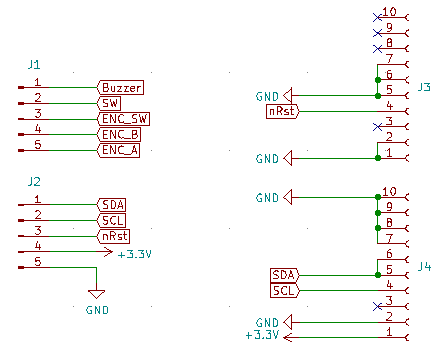
\includegraphics[width=.75\textwidth]{sec6/images/Display_PCB} 
\centering
\captionsetup{width=.95\textwidth}
\caption[Schaltplan des Bedienungs-Boards 1]{Schaltplan des Bedienungs-Boards mit den Stiftleisten J1 und J2 zur Verbindung mit dem Mikrocontroller und den Buchsenleisten J3 und J4 für das Display}\centering
\label{fig:BedienungsBoard1}
\end{figure}

\begin{figure}[H] %H für Positionierung hier
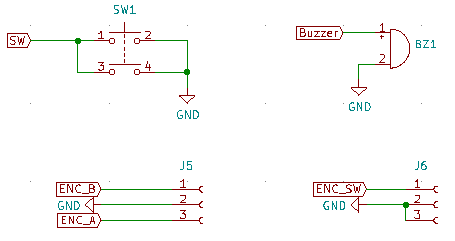
\includegraphics[width=.90\textwidth]{sec6/images/Display_PCB2} 
\centering
\captionsetup{width=.95\textwidth}
\caption[Schaltplan des Bedienungs-Boards 2]{Schaltplan des Bedienungs-Boards mit dem Drehencoder, dem Taster und dem Summer}\centering
\label{fig:BedienungsBoard2}
\end{figure}


\subsection{Programmierung der Anzeige}\label{Sec6Sub2}
***HIAS***


\subsection{Programmierung der Steuerelemente}\label{Sec6Sub3}
***HIAS***



\newpage